Um einen geeigneten Filter im Sinne

\section{Mathematische Idee} \label{sec:math}%vorher "Hintergrund" eher fuer BA geeignet
\textcolor{red}{JORDAN KURVE?}
Zun"chst wollen wir uns mit den mathematischen Ideen, welche die
Grundlage f"ur den \textsc{FEAST}-Algorithmus bilden, vetraut machen. Daf"ur werden wir
die von E. Polizzi in seinem Paper~\cite{polizzi} verwendeten Notationen in gro"sen
Teilen -- aber nicht vollst"andig -- "ubernehmen.\\

Es seien nun zwei  Zahlen $\lambda_1, \lambda_2 \in \R$ vorgegeben, die
das reelle Intervall $I:=[\lambda_1, \lambda_2] \subseteq \R$ definieren.
F"ur zwei hermitesche Matrizen $A, B \in \Cnn$ mit der zus"atzlichen
Forderung, dass $B$ positiv definit ist, sollen Paare der Gestalt
$(\lambda, x) \in I \times \C^n$ ermittelt werden, welche der verallgemeinerten
Eigenwertgleichung

  \begin{equation}\label{eq:eigen} %eventuell einfaches ewp
  Ax = \lambda Bx
  \end{equation}

gen"ugen. Um diese Eigenpaare\footnote{Um der besseren Lesbarkeit Willen werden
im Folgenden die verallgemeinerten Eigenvektoren und deren verallgemeinerte
Eigenwerte kurz als Eigenvektor und Eigenwert bezeichnet.}
bestimmen zu k"onnen, wird das Problem mit Hilfe einer
gewissen Matrix $Q\in\Cnn$ in das "aquivalente Problem

  \begin{equation}\label{eq:Qeigen}
  A_Q \phi = \mu B_Q \phi
  \end{equation}

"uberf"uhrt. Hierbei sind $A_Q = Q^TAQ$, $B_Q = Q^TBQ$ und $(\mu, \phi)
\in I\times\C^n$.
Wird die Matrix $Q$ richtig gew"ahlt, so ist dann jeder zul"assige Eigenwert von
\eqref{eq:Qeigen} auch ein zul"assiger Eigenwert von \eqref{eq:eigen} und
umgekehrt.\footnote{Daher ist die Angabe $\mu\in I$ gerechtfertigt.}
F"ur die Ermittlung der gesuchten Eigenvektoren bedarf es hingegen zus"atzlicher Arbeit.\\

Zur Bestimmung der Transformationsmatrix $Q$ wird eine Konturintegration bem"uht.
Ausgangspunkt dieser Integration ist die durch

  \begin{align*}
  G\colon\Omega &\to\Cnn\\
  \omega &\mapsto (\omega B - A)^{-1}
  \end{align*}

definierte  \textsc{Green}-Funktion, wobei $\Omega \subseteq \C$ eine passende
Teilmenge der komplexen Zahlen ist. Insbesondere m"ussen $\Omega$ und das
Spektrum von $B^{-1}A$ disjunkt sein, da $G$ andernfalls nicht wohldefiniert ist.\\

Die Funktion $G$ wird nun "uber eine geschlossene komplexe Kurve $\gamma$,
die um das vorgegebene Intervall $I$ heruml"auft, in der Gestalt
\[
-\frac{1}{2\pi\iota}\int_\gamma G(\omega)\text{ d}\omega
\]
integriert.\footnote{Mit $\iota$ ist im Folgenden stets die imagin"are Einheit bezeichnet,
also $\iota = \sqrt{-1}$.}\\

Wir wollen nun annehmen,
dass es genau $k\in\N$ Eigenwerte gibt,
die im Inneren des Intervalls $I$ liegen.\footnote{Diese Forderung ist wohldefiniert, da
der Eigenschaften von $A$ und $B$ wegen alle Eigenwerte von $B^{-1}A$ reell sind.}
F"ur zu diesen Eigenwerten passende Eigenvektoren $\{x_i\}_{i=1:k} \subseteq \Cn$ sei au"serdem die Matrix
$X_k := [x_i]_{i=1:k}$ gegeben.
Dann l"asst die Konturintegration R"uckschl"usse auf die Eigenvektoren zu, denn man kann
zeigen, dass die Identit"at
\begin{equation}\label{eq:integral}
X_k X_k^T = \sum_{i=1}^k x_i x_i^T =
-\frac{1}{2\pi\iota}\int_\gamma G(\omega)\text{ d}\omega
\end{equation}
gilt.\\

Wir w"ahlen nun $k$ linear unabh"angige Vektoren $\{y_i\}_{i=1:k} \subseteq \Cn$
aus, die wir in der Matrix $Y_k := [ y_i ]_{i=1:k}$ zusammenfassen.
Unsere gew"unschte Matrix $Q$ definieren wir nun durch Matrixmultiplikation
verm"oge
\begin{equation}\label{eq:Q}
Q := X_k X_k^T Y_k.
\end{equation}
Die Spalten von $Q$ sind also gerade Linearkombinationen aus den Eigenvektoren.
Sind dann $\{\phi_i\}_{i=1:k} \subseteq \Cn$ Vektoren die das transformierte
Eigenwertproblem \eqref{eq:Qeigen} l"osen
und ist $\Phi_k:=[\phi_i]_{i=1:k}$ gegeben,
so gilt $X_k = Q \Phi_k$.\\

In der Praxis sind nat"urlich weder die Anzahl der Eigenwerte noch die dazugeh"origen Eigenvektoren
bekannt. W"ahrend die Anzahl mit Hilfe einer passenden Filterfunktion bestimmt werden kann,
verhilft die wegen \eqref{eq:integral} und \eqref{eq:Q} g"ultige Gleichheit
\begin{equation}\label{eq:solution}
Q = -\frac{1}{2\pi\iota}\left(\int_\gamma G(\omega)\text{ d}\omega\right)\cdot Y
\end{equation}
zur Berechnung der Eigenvektoren.

%B-Orthogonalit"at der x-vektoren
\newpage
\section{Beispiel}\label{sec:bsp}

In diesem Abschnitt soll mit Hilfe eines einfachen Beispiels die eben erarbeitete
Theorie verifiziert werden. Daf"ur betrachten wir die beiden Matrizen
$A,B \in \Cnn$, welche durch
\[
A:= \begin{bmatrix} 0 & 0 & 0 \\ 0 & 1 & 0 \\ 0 & 0 & -1 \end{bmatrix} \text{ und }
B:= \begin{bmatrix} 1/2 & 0 & 0\\ 0 & 1/2 & 0 \\ 0 & 0 & 1/4 \end{bmatrix}
\]
gegeben sind. Durch einfaches Nachrechnen "uberpr"uft man, dass das
verallgemeinerte Eigenwertproblem \eqref{eq:eigen} durch Vektoren
$x_1 \in \spn_\C\{e_1\}$ mit zugeh"origem Eigenwert $\lambda_1 = 0$, Vektoren
$x_2 \in \spn_\C\{e_2\}$ mit zugeh"origem Eigenwert $\lambda_2 = 2$, sowie
Vektoren $x_3 \in\spn_\C\{e_3\}$ mit zugeh"origem Eigenwert $\lambda_3 = -4$
gel"ost wird.\footnote{Hier bezeichnen $e_1, e_2, e_3 \in\Cn$ die kanonischen Einheitsvektoren.}\\

Wir wollen nun auf dem reellen Intervall $[-3,3]$ die Eigenpaare bestimmen.
Als Integrationskontur w"ahlen wir daher den Kreis mit einem Radius von drei
L"angeneinheiten und dem Mittelpunkt im Ursprung. Das hei"st, wir werden die
\textsc{Green}-Funkion $G$ "uber die Kurve
\begin{equation}\label{kurve}
\gamma\colon [0,2\pi]\to\Cn\text{, }\varphi\mapsto 3e^{\iota \varphi}
\end{equation}
integrieren. Da nach Konstruktion keiner der Eigenwerte auf dem
Graphen von $\gamma$ liegt, ist $G$ auf der gesamten Kontur wohldefiniert.

\begin{figure}[h!]
	\center
	\begin{tikzpicture}
	\draw[->] (-3.5cm,0cm) -- (3.5cm,0cm) node[right,fill=white] {Re};
    \draw[->] (0cm,-2.5cm) -- (0cm,2.5cm) node[above,fill=white] {Im};
    \draw[->] (0cm, 0cm) -- (1.41, 1.41);
	\draw[red](0cm,0cm)circle(2cm);
	\foreach \x in {-3,0,1.33} {
	\filldraw[black] (\x cm,0) circle(2pt);
	}
	\draw (0.3,-0.3) node{$\lambda_1$};
	\draw (1.33,-0.3) node{$\lambda_2$};
	\draw (-3,-0.3) node{$\lambda_3$};
	\node[rotate=45] at (0.5, 1) {$r=3$};
	%\node at (2.3,-2.3) {$\C$};
	\end{tikzpicture}
	\caption{Skizze der Kurve \textcolor{red}{$\gamma$} in der komplexen Ebene.}
\end{figure}

Zun"achst "uberpr"ufen wir
die Identit"at \eqref{eq:integral}. Mit $x_1 := \begin{bmatrix} \sqrt2 \iota & 0 & 0
\end{bmatrix}^T$
und $x_2 := \begin{bmatrix} 0 & \sqrt2 \iota &0\end{bmatrix}^T$ sind zwei passende
Eigenvektoren f"ur unser Eigenwertproblem gegeben, und in der Tat gilt
\begin{align*}
-\frac{1}{2\pi\iota} \int_\gamma G(\omega) \text{ d}\omega &=
-\frac{1}{2\pi\iota}\int_0^{2\pi} G(\gamma(\omega))\cdot \gamma'(\omega)
\text{ d}\omega \\
&= -\frac{1}{2\pi\iota}\int_0^{2\pi} \begin{bmatrix} \frac{2}{3e^{\iota\omega}}&0&0\\
0 & \frac{2}{3e^{\iota\omega}-2}&0\\
0&0&\frac{4}{3e^{\iota\omega}+4}
 \end{bmatrix}\cdot 3\iota e^{\iota\omega}
\text{ d}\omega \\
&= \text{diag}(-2,-2,0) \\
&= x_1 x_1^{T} + x_2 x_2^T.
\end{align*}

Als N"achstes "uberpr"ufen wir, ob die Matrix $X_2 := \begin{bmatrix} x_1 & x_2\end{bmatrix}$ mit Hilfe der in Abschnitt \ref{sec:math} beschriebenen Methode rekonstruierbar ist.\\

Dort wird von uns zun"achst die Konstruktion der Matrix $Q$ aus \eqref{eq:Q} verlangt.
Da wir bereits wissen, dass wir zwei Eigenvektoren finden wollen, w"ahlen wir also beliebig
eine Matrix $Y_2 \in \C^{3,2}$ vollen Ranges -- die wir in diesem
Beispiel mit $Y_2 := \begin{bmatrix} e_1 & e_1 + e_2 \end{bmatrix}$ festlegen wollen --
und multiplizieren diese von rechts an das Integral der \textsc{Green}-Funktion "uber
die durch \eqref{kurve} definierte Kontur.\footnote{Es mag den Leser verwundern,
wie bei Unkenntnis "uber die Anzahl $k\in\N$ der zu findenden Eigenvektoren die
Spaltenzahl von $Y_k$ korrekt zu ermitteln ist. Eine g"angige Methode ist zum Beispiel das Konstruieren einer
passenden Filterfunktion, welche die nicht erw"unschten Eigenwerte aussortiert (Vgl. Abschnitt \ref{sec:rkt}).}
Wir erhalten somit
\[
Q = -\frac{1}{2\pi\iota}\left(\int_{\gamma}G(\omega)\text{ d}\omega \right)\cdot Y_2
= \begin{bmatrix} -2 & 0&0 \\ 0 & -2& 0\\ 0&0&0\end{bmatrix}
\begin{bmatrix} 1 & 1 \\ 0 & 1\\0&0 \end{bmatrix}
= \begin{bmatrix} -2 & -2 \\ 0 & -2\\0&0 \end{bmatrix}.
\]
Nun l"osen wir das in \eqref{eq:Qeigen} beschriebene
Eigenwertproblem. Wir suchen also Paare $(\mu,\phi) \in \C\times\Cn$ die
der Gleichung
\[
A_Q \phi = \mu B_Q \phi
\]
gen"ugen. Durch Nachrechnen "uberzeugt man sich davon, dass dieses von allen
Vektoren $\phi_1 \in \spn_\C\{e_1\}$ mit dem Eigenwert $\mu_1 = 0$ sowie
allen Vektoren $\phi_2 \in \spn_\C\{-e_1 + e_2\}$ mit dem Eigenwert
$\mu_2 = 2$ gel"ost wird.\\

Die soeben ermittelten Eigenwerte stimmen also schon mit den Eigenwerten
unseres betrachteten Problems "uberein. W"ahlen wir schlie"slich die Matrix
\[
\Phi_2 := \begin{bmatrix} \phi_1 & \phi_2 \end{bmatrix} :=
\begin{bmatrix} -\iota/\sqrt2  & \iota/\sqrt2 \\ 0 & -\iota/\sqrt2 \end{bmatrix},
\]
mit den Eigenvektoren $\phi_1$ und $\phi_2$, so erhalten wir wie gew"unscht
\[
Q\Phi_2 = \begin{bmatrix} -2 & -2 \\ 0 & -2\\0&0 \end{bmatrix}
\begin{bmatrix} -\iota/\sqrt2  & \iota/\sqrt2 \\ 0 & -\iota/\sqrt2 \end{bmatrix} =
\begin{bmatrix} \sqrt2 \iota & 0 \\ 0 & \sqrt2 \iota \\ 0 &0\end{bmatrix} = X_2.
\]

\textbf{Bemerkung.} An dieser Stelle sei darauf hingewiesen,
dass die Matrix $\Phi_2$ aus kosmetischen Gr"unden gerade so
gew"ahlt wurde, dass die Kalkulation am Ende $X_2$ ergibt und somit alles
h"ubsch anzusehen ist.
Der Wahl einer anderen Matrix $\Phi'_2$ mit skalaren Vielfachen der hier
gew"ahlten Eigenvektoren steht selbstverst"andlich nichts im Wege und f"uhrt freilich zu einer anderen
Matrix $X_2'$, deren Spalten ebenfalls zul"assige Eigenvektoren enth"alt.\\


% (4) Implementation

\section{Realisierung des FEAST-Algorithmus'}

Nun, da die mathematischen Ideen diskutiert und durch ein Bespiel verifiziert
worden sind, widmen wir uns der Implementation des FEAST-Algorithmus' in MATLAB.
Wir orientieren uns dabei an der Vorgehensweise aus dem Beispiel in Abschnitt
\ref{sec:bsp}. Auch die Notation wird beibehalten.

\subsection{Naive Implementation}
Zun"achst w"ahlen wir also f"ur $k\in\N$ eine vollrangige Zufallsmatrix $Y_k$, um
die Transformationsmatrix $Q$ zu ermitteln. Dazu f"uhren wir die \textsc{Green}-Funktion
\[
\mcode{funGreen = @(w) inv( w.*B-A )}
\]
ein und w"ahlen eine passende Integrationskontur
$C$. Um es einfach zu halten, wird diese in der Implementation die Menge
\[
C = \left\{ z \in \C : \left\lVert z - \frac{\lambda_\text{max} -
\lambda_\text{min}}{2} \right\rVert_1\ = 1\right\}
\]
sein, wobei $\lambda_\text{min}$ und $\lambda_\text{max}$ die vorgegebenen Intervallgrenzen
bezeichnen. Die entsprechenden Quadraturpunkte werden im Quellcode durch die
Variablen
\[
\mcode{n0, n1, n2, n3}
\]
repr"asentiert.\\

Ist $Q$ bestimmt, benutzen wir die MATLAB interne Eigenwertfunktion
\[
\mcode{eig(Aq, Bq)}
\]
um die \textsc{Ritz}-Paare des transformierten Problems zu berechnen. Schlie"slich
berechnen wir die Eigenwerte und Eigenvektoren des urspr"unglichen Problems.
Die Matrix $\Phi_k$ wird im Quelltext mit  \mcode{Vq} bezeichnet.\\

Wir wollen annehmen, dass der Input des Users die Voraussetzungen des
Problems \eqref{eq:eigen} erf"ullt und die Anzahl $k\in\N$ der Eigenwerte
im Intervall $[\lambda_\text{min}, \lambda_\text{max}]$ bekannt ist.
Eine naive Implementation k"onnte daher wie folgt aussehen:

\begin{lstlisting}[caption=Naive FEAST Implementation., captionpos=b]
%% Eingabe: Matrizen A, B des Eigenwertproblems,
%%          Intervallgrenzen lmin, lmax,
%%	        Anzahl k der erwarteten Eigenwerte
%% Ausgabe: Matrix V mit Eigenvektoren,
%%          Matrix D mit Eigenwerten auf der Diagonalen

%% Funktionsaufruf: [V, D] = feast[A, B, lmin, lmax, k]

function[V, D] = feast(A, B, lmin, lmax, k);

n = length(A);

% erzeuge Zufallsmatrix
Y = randn(n, k);

% generiere Green-Funktion
funGreen = @(w) inv( w.*B - A );

% berechne die Integrationsknotenpunkte
n0 = lmax;
n1 = (lmin + lmax)/2 + (lmax - (lmin + lmax)/2)*i;
n2 = lmin;
n3 = (lmin + lmax)/2 - (lmax - (lmin + lmax)/2)*i;

% Integrationskontur
C = [n1 n2 n3];

% berechne Transformationsmatrix Q
Q = (-1/(2*pi*i))*integral(funGreen, n0, n0,...
	'Waypoints', C, 'ArrayValued', true) * Y;

% berechne Ritz-Paare des transformierten Problems
Aq = Q'*A*Q; Bq = Q'*B*Q;
[Vq, D] = eig(Aq, Bq);

% berechne die gesuchten Eigenvektoren
V = Q*Vq;
\end{lstlisting}

"Uberpr"ufen wir die Funktionalit"at mit den Matrizen $A$ und $B$ aus dem Abschnitt
\ref{sec:bsp}, erhalten wir folgende Ausgabe:

\begin{lstlisting}[numbers=none]
>> [V, D] = feast(A, B, -3, 3, 2)

V =

  -1.4142 - 0.0000i   0.0000 + 0.0000i
   0.0000 + 0.0000i   1.4142 - 0.0000i
  -0.0000 + 0.0000i  -0.0000 + 0.0000i


D =

    0.0000         0
         0    2.0000

>>
\end{lstlisting}

\vspace{0.5cm}
Die vorgestellte Umsetzung des FEAST-Algorithmus' l"asst sich ohne Weiteres auf
dynamische Matrixdimensionen "ubertragen. Da sich mit zunehmender Dimension
unter Umst"anden auch die Kardinalit"at des Spektrums und die Anzahl der Eigenr"aume "andert, sollten
gegebenenfalls Optimierungsma"snahmen getroffen werden, wie etwa die Wahl der Knotenpunkte f"ur die
Konturintegration.\\

Man k"onnte sich nun die Frage stellen, warum man anstatt \eqref{eq:eigen} nicht
einfach das Problem
\[
B^{-1}Ax = \lambda x
\]
zu l"osen versucht. Der positiven Definitheit von $B$ wegen, w"are diese
Umformulierung m"oglich und mit bek"ommlicheren Verfahren l"osbar. \\

Nun ist aber das Invertieren von Matrizen bekannterma"sen numerisch
eher ung"unstig, da man unter Umst"anden mit hohem Rechenaufwand
und dem Verlust von Stabilit"at bezahlen muss. Ein erneuter Blick
auf \eqref{eq:integral} oder \eqref{eq:Q} stimmt demnach benklich,
da sowohl mit der Integration als auch mit dem Berechnen der \textsc{Green}-Funktion
gewisse Risiken eingegangen werden.\\

Man muss sich also die Frage stellen, ob eine Implementation des FEAST-Algorithmus
ohne Inversion und Integration m"oglich ist.

%(4) RKToolbox%

\subsection{Rational Krylov Toolbox}\label{sec:rkt}

Wie in der Einleitung versprochen, soll abschlie"send ein numerischer Werkzeugkoffer
pr"asentiert werden, der es erm"oglicht den FEAST-Algorithmus elegant und ohne
die eben beschriebenen Bedenklichkeiten umzusetzen.\\

Mit der \glqq\emph{Rational Krylov Toolbox for MATLAB}\grqq\ ~\cite{RKT} stellen deren Entwickler
\textsc{Mario Berljafa} und \textsc{Stefan G"uttel} eine Bibliothek zur Verf"ugung, die es erm"oglicht, g"angige \textsc{Krylov}-Unterraum-Verfahren unkompliziert zu implementieren.
Bevor wir dieses Tool genauer betrachten, wollen wir uns klarmachen, warum
die Anwendung eines solchen Verfahrens m"oglich ist.  Dazu
begn"ugen wir uns an dieser Stelle mit einer Plausibilit"atsbetrachtung.\\

Studieren wir erneut die in \eqref{eq:integral} formulierte Identit"at
\[
X_k X_k^T := \sum_{i=1}^k x_i x_i^T =
-\frac{1}{2\pi\iota}\int_\gamma G(\omega)\text{ d}\omega,
\]
f"allt sodann auf, dass die Abbildung
\[
P\colon \Cn\to\Cn,
v\mapsto Pv := \left(-\frac{1}{2\pi\iota}\int_\gamma G(\omega)\text{ d}\omega\right)v
\]
Vektoren in den von den Eigenvektoren $(x_i)_{1:k}$ aufgespannten Unterraum abbildet.
Man kann sogar zeigen, dass die Abbildung eine $B$-orthogonale Projektion ist. Die Idee, den
FEAST-Algorithmus per Projektionsverfahren umzusetzen, liegt demnach gar nicht so fern.\\

Eine m"ogliche Implementation stellen die Autoren in ihren Beispielen auf der Seite
\begin{center}
\small
\url{http://www.guettel.com/rktoolbox/examples/html/example_feast.html}
\end{center}

vor:

\begin{lstlisting}[caption=FEAST-Implementation mit Unterraumprojektion., captionpos=b]
% Search space basis V of dimension m.
m = 10;
V = randn(N, m);

for iter = 1:8
  % Apply rational filter to V.
  V = r(A, V);
  % Compute and sort Ritz pairs.
  Am = V'*A*V; Bm = V'*B*V;
  [W, D]   = eig(Am, Bm);
  [D, ind] = sort(diag(D)); W = W(:, ind);
  % B-normalize W.
  nrm = sqrt(diag(W'*Bm*W)); W = W/diag(nrm);
  % Form approximate eigenvectors.
  V = V*W;
  % Check residuals and number of eigenpairs inside
  % search iterval.
  Di = diag(D(lmin < D & D < lmax));
  Vi = V(:, lmin < D & D < lmax);
  resid(iter) = norm(A*Vi - B*Vi*Di, 'fro');
  nrvec(iter) = size(Vi, 2);
end
\end{lstlisting}

Diese beginnt mit der Initialisierung und dem Festlegen eines Suchraums, der durch die Spalten der Matrix
$V$ aufgespannt wird. Hierbei ist $N$ die Dimension der Matrizen $A$ und $B$ und $m$ die Anzahl der
erwarteten Eigenpaare.\footnote{Auch in diesem Beispiel ist diese Anzahl der Eigenpaare im Voraus bekannt.
Trotzdem wird ein Filter eingesetzt.}\\

In der folgenden Iterationsschleife wird der Eigenraum approximiert. Besonderes Augenmerk muss auf die
Filterfunktion \mcode{r} gelegt werden. Diese ist gerade so konzipiert, dass Argumente innerhalb des
Suchintervalls in einen Bereich $(1-\varepsilon, 1+\varepsilon)$ abbgebildet werden. Der Wert $\varepsilon > 0$ ist
hierbei vom Input abh"angig und kann stark variieren. Argumente au"serhalb des Intervalls werden in "ahnlicher
Manier auf einen Bereich $(-\delta, \delta)$ abgebildet -- f"ur ein entsprechendes $\delta > 0$.

\begin{figure}[h!]

    \centering

    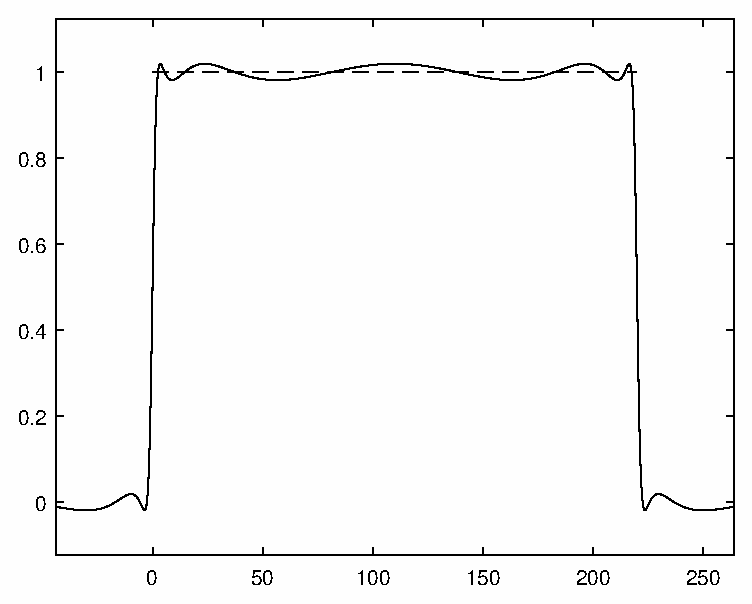
\includegraphics{images/epsFig}

    \caption{Filterfunktion \mcode{r} auf dem Intervall [0,220] wirkend.}

\end{figure}

Der Toolbox-interne Aufruf \mcode{r(A,V)} erm"oglicht nun das Berechnen der Wirkung des Filters
auf den Suchraum $V$.\\

Schlussendlich l"ost der Algorithmus auch hier das transformierte Eigenwertproblem und ermittelt daraus
approximativ die gesuchten Eigenpaare.
